\clearpage
%%=========================================
% Den litt rare section-formuleringen er for å en kortere header-tittel siden den er for lang ellers.
% \sectionmark{} inne i {section title as seen in paper ...} er for å få riktig header der en section begynner på en oddetallsside.
%
%   \section[section title as seen in TOC]{section title as seen in paper%
%       \sectionmark{section title as seen in header}}\sectionmark{section title as seen in header}
%
\section[Surface Analysis of Substrate A with Surface Pre-Growth Preparation]{Surface Analysis of Substrate A with Surface Pre-Growth Preparation%
    \sectionmark{Surface Analysis of Pre-Growth Substrate A}}\sectionmark{Surface Analysis of Pre-Growth Substrate A}\label{sec:subAb}


%%=========================================
\subsection{Particles}

\begin{figure}
    \centering
    \begin{subfigure}[t]{\textwidth}
          \begin{minipage}[t]{0.49\linewidth}
            \centering
            
\includegraphics[width=\linewidth]{unknown.png}
          \end{minipage}
          \hspace{0.02\linewidth}
          \begin{minipage}[t]{0.49\linewidth}
            \centering
            
\includegraphics[width=\linewidth]{unknown.png}
          \end{minipage}
        \caption{\todo{Add caption}}\label{fig:add_label}
    \end{subfigure}
    \par\bigskip
    \begin{subfigure}[t]{\textwidth}
          \begin{minipage}[t]{0.49\linewidth}
            \centering
            
\includegraphics[width=\linewidth]{unknown.png}
          \end{minipage}
          \hspace{0.02\linewidth}
          \begin{minipage}[t]{0.49\linewidth}
            \centering
            
\includegraphics[width=\linewidth]{unknown.png}
          \end{minipage}
        \caption{\todo{Add caption}}\label{fig:add_label}
    \end{subfigure}
    \par\bigskip
    \begin{subfigure}[t]{\textwidth}
          \begin{minipage}[t]{0.49\linewidth}
            \centering
            
\includegraphics[width=\linewidth]{unknown.png}
          \end{minipage}
          \hspace{0.02\linewidth}
          \begin{minipage}[t]{0.49\linewidth}
            \centering
            
\includegraphics[width=\linewidth]{unknown.png}
          \end{minipage}
        \caption{\todo{Add caption}}\label{fig:add_label}
    \end{subfigure}
    \caption[\Ac{sem} images and \ac{eds} spectra of particles found on substrate A after surface pre-growth preparation.]{High resolution \acf{sem} images of particles found on substrate A after surface pre-growth preparation and the corresponding \acf{eds} spectra of the particles.}\label{fig:subAb_sem_w_eds}
\end{figure}

\begin{figure}[htbp]
\ContinuedFloat
    \centering
    \begin{subfigure}[t]{\textwidth}
          \begin{minipage}[t]{0.49\linewidth}
            \centering
            
\includegraphics[width=\linewidth]{unknown.png}
          \end{minipage}
          \hspace{0.02\linewidth}
          \begin{minipage}[t]{0.49\linewidth}
            \centering
            
\includegraphics[width=\linewidth]{unknown.png}
          \end{minipage}
        \caption{\todo{Add caption}}\label{fig:add_label}
    \end{subfigure}
    \captionsetup{list=no}
    \caption{\emph{(continued)}}
\end{figure}


%%=========================================
%\section{AFM Study of Etched Substrate A}
\subsection{Surface Roughness}

\begin{figure}[htbp]
    \centering
    \begin{subfigure}[t]{\linewidth}
        \centering
        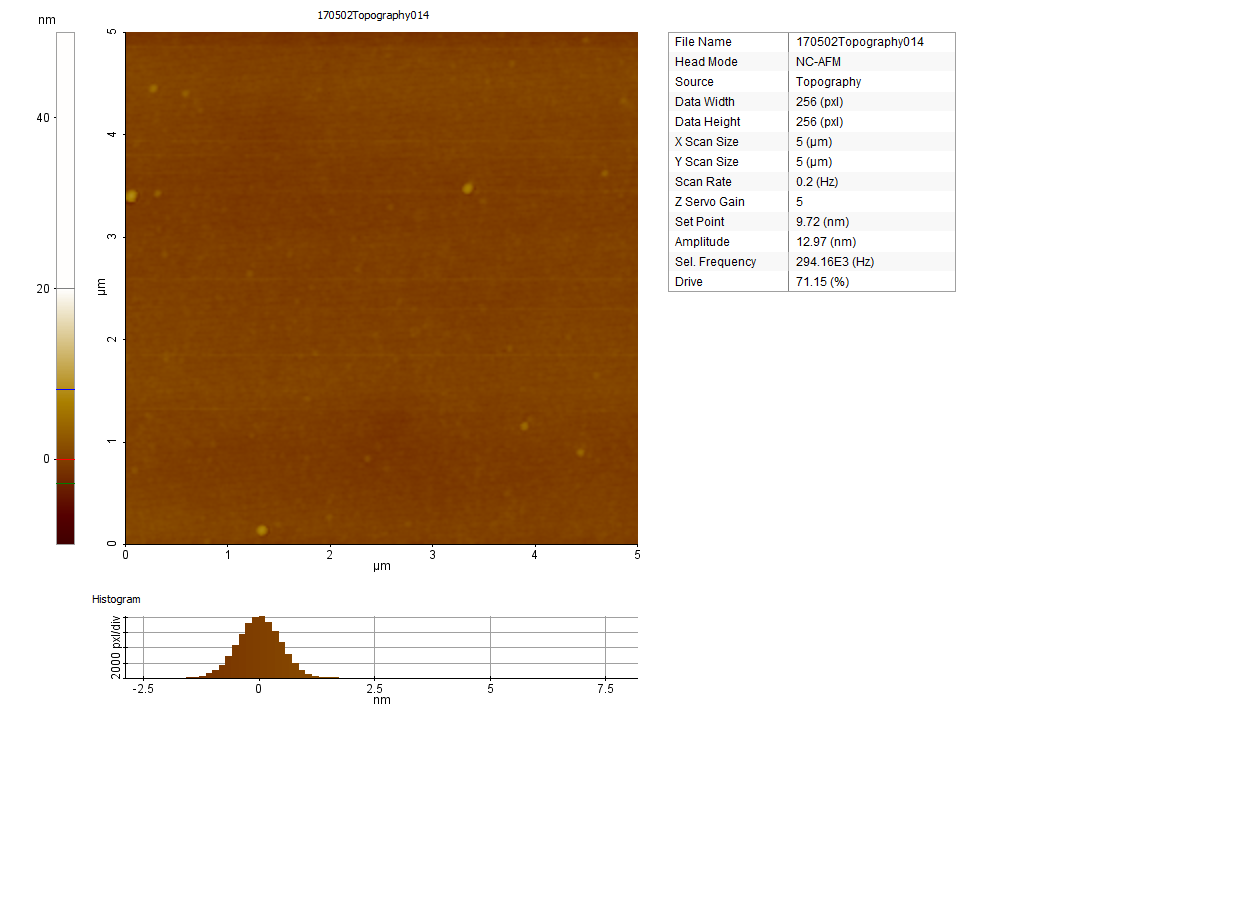
\includegraphics[width=0.5\linewidth,trim={0cm 12cm 21cm 0cm},clip]{170502Topography014_centre.png}
        \caption{Near centre, \ac{rms} roughness \SI{0.51}{\nano\metre}.} %\SI{0.85}{\nano\metre}
    \end{subfigure}%
    \par\bigskip
    \begin{subfigure}[t]{\linewidth}
        \centering
        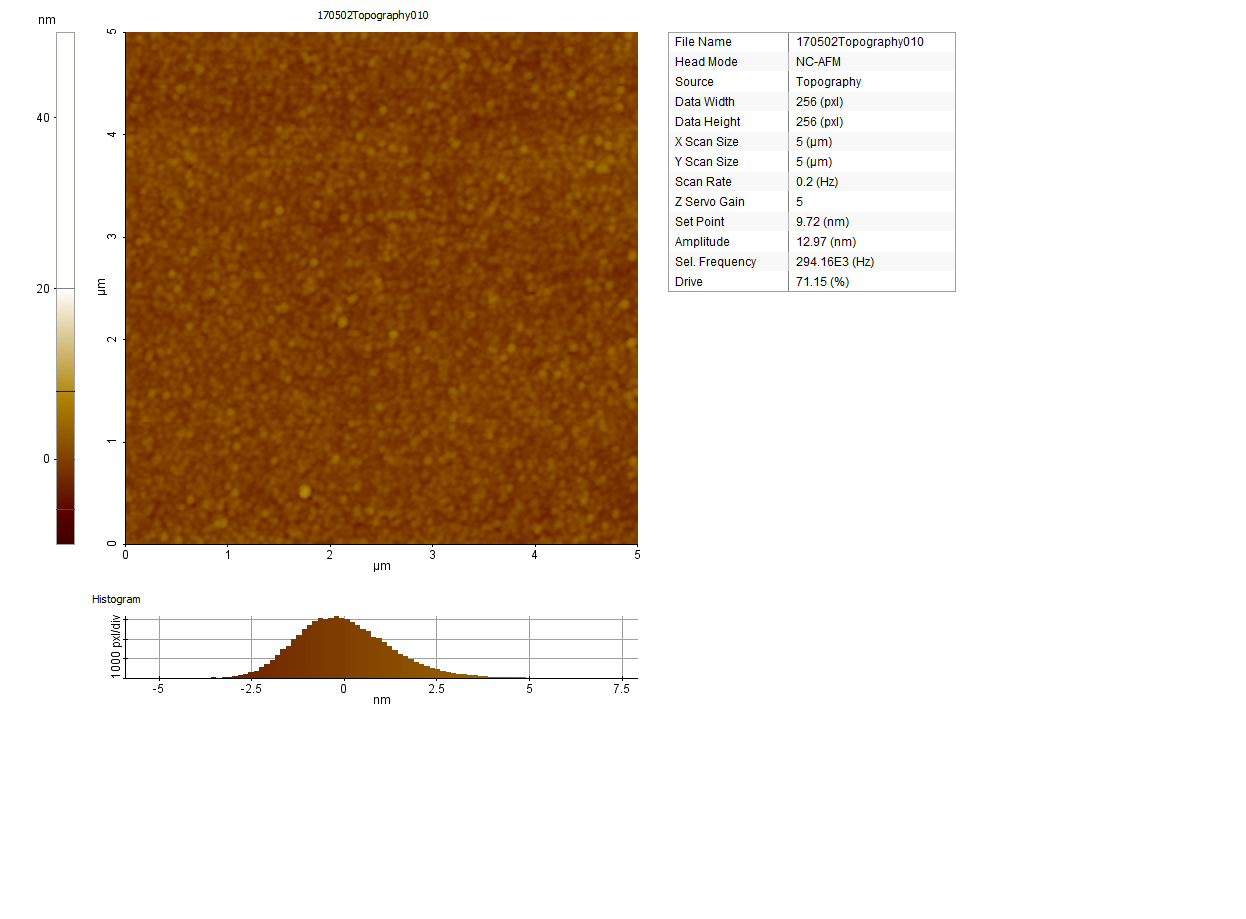
\includegraphics[width=0.5\linewidth,trim={0cm 12cm 21cm 0cm},clip]{170502Topography010_upperedge.png}
        \caption{Near upper edge, \ac{rms} roughness \SI{1.3}{\nano\metre}.} %\SI{0.77}{\nano\metre}}
    \end{subfigure}%
    \par\bigskip
    \begin{subfigure}[t]{\linewidth}
        \centering
        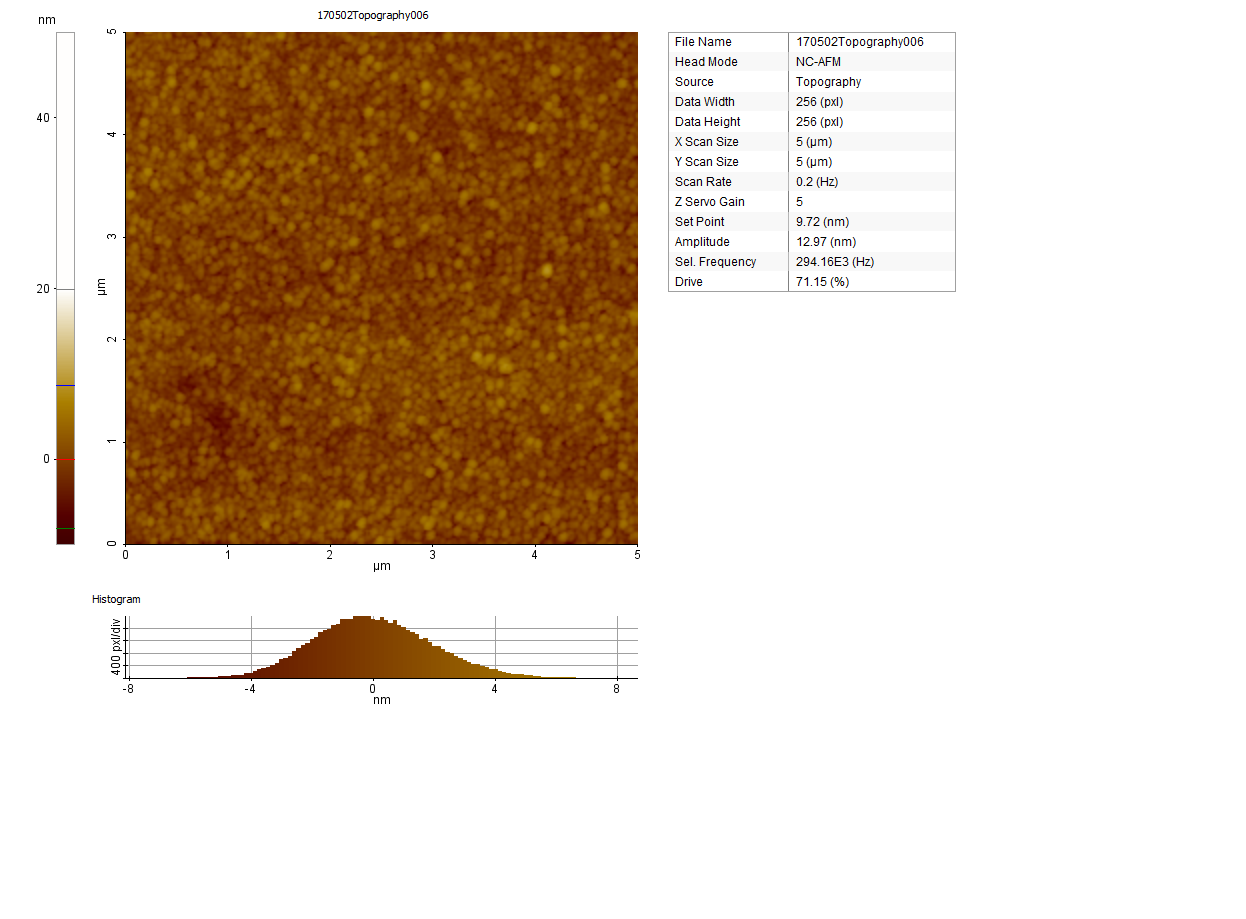
\includegraphics[width=0.5\linewidth,trim={0cm 12cm 21cm 0cm},clip]{170502Topography006_upperleftcorner.png}
        \caption{Near upper left corner, \ac{rms} roughness \SI{1.9}{\nano\metre}.}\SI{1,04}{\nano\metre}
    \end{subfigure}%
    \caption[\Ac{afm} of substrate A with surface pre-growth preparation.]{\Acf{afm} measurements of substrate A with surface pre-growth preparation. Images of a $\SI{5}{\micro\metre}\times\SI{5}{\micro\metre}$ area are taken at the centre, edge, and corner of the substrate.}\label{fig:afm_subAb}
\end{figure} % AFM, substrate A, with surface pre-growth preparation.

%%=========================================
\subsection{Impurity Analysis}

\begin{table}[htbp]
    \centering
    \caption[\Ac{eds} impurity analysis of substrate A with surface pre-growth preparation.]{Results of the \acf{eds} impurity analysis at three different locations on the $30\times30$ \SI{}{\milli\metre^2} (111)B \ac{czt} substrate A with surface pre-growth preparation (atomic concentration \%). The X-ray signal is acquired from a $\SI{1270}{}\times\SI{890}{\micro\metre^2}$ area centred around the given $X$ and $Y$ values at a magnification of 100$\times$.}\label{tab:subAb_eds_analysis}
   \begin{tabu} to 1.0\textwidth { X[1,c] X[1,c] X[1.125,c] X[1.125,c] X[1.125,c] X[1.125,c] X[1.125,c] X[1.125,c] X[1.125,c] }
    \hline
        \textbf{$X$} (\SI{}{\milli\metre}) &  \textbf{$Y$} (\SI{}{\milli\metre}) & \textbf{\ce{Te}} (at.\%) & \textbf{\ce{Cd}} (at.\%) & \textbf{\ce{Zn}} (at.\%) & \textbf{\ce{Al} } (at.\%) & \textbf{\ce{Si}} (at.\%) & \textbf{\ce{C}} (at.\%) & \textbf{\ce{O}} (at.\%) \\
        \hline
         \SI{1.0}{}  & \SI{29.0}{} & \SI{}{} & \SI{}{} & \SI{}{} & \SI{}{} & \SI{}{} & \SI{}{} & \SI{}{} \\
         \SI{15.0}{} & \SI{29.0}{} & \SI{}{} & \SI{}{} & \SI{}{} & \SI{}{} & \SI{}{} & \SI{}{} & \SI{}{} \\
         \SI{15.0}{} & \SI{15.0}{} & \SI{}{} & \SI{}{} & \SI{}{} & \SI{}{} & \SI{}{} & \SI{}{} & \SI{}{} \\
         \hline
    \end{tabu}
\end{table}
%%=========================================

